\chapter{DSP setup}

In this chapter the setup of the DSP is explained. 

\section{DSP setup}

The initialization is performed in a function called system\_init, which is shown in \autoref{listingSystemInit}. The first two lines of the function is the setup of the clock. SYS\_PCGCR1 and SYS\_PCGCR2 are defined as IO-ports to the registers namely 0x1c02 and 0x1c03. By setting SYS\_PCGCR1 and SYS\_PCGCR2 (Peripheral Clock Gating Configuration Registers) to 0 the clock is activated on all peripherals needing a clock. The next line SYS\_EXBUSSEL, which has the IO register address 0x1c00, is the external bus selector. The register determine which of the external peripheral IO unit is selected. By setting the register to 0x1100, SPI, GPIO, UART, I2S2 and I2S0 and, are activated. The system only uses the I2S0 and UART ports. The I$^2$C is afterwards initialized. The I$^2$C bus is used for communication between the TMS320C5515 and TLV320AIC3204.

\begin{lstlisting}[language=C, caption = {System initialization},label={listingSystemInit}]
void system_init(uint8 audioType, uint8 resolution, uint8 fs){
    SYS_PCGCR1 	 = 0x0000;     		/* Enable clocks to all peripherals */
    SYS_PCGCR2 	 = 0x0000;
	SYS_EXBUSSEL = 0x1100;         	// Enable I2S bus
	I2C_init();        				// Initialize I2C
	
	if 		(fs == 48 && resolution == 16) TLV320AIC3204_init(0x0d, 0x07, 0x06, 0x90);
	else if (fs == 48 && resolution == 24) TLV320AIC3204_init(0x2d, 0x07, 0x06, 0x90);	
	else if (fs == 96 && resolution == 16) TLV320AIC3204_init(0x0d, 0x0E, 0x0D, 0x20);	
	else if	(fs == 96 && resolution == 24) TLV320AIC3204_init(0x2d, 0x0E, 0x0D, 0x20);
	else TLV320AIC3204_init(0x0d, 0x07, 0x06, 0x90);	
	
	wait(200);        				// Wait	
	if 		(audioType == 0 && resolution == 16) I2S_init(0x9010);
	else if (audioType == 0 && resolution == 24) I2S_init(0x901C);	
	else if (audioType == 1 && resolution == 16) I2S_init(0x8010);	
	else if	(audioType == 1 && resolution == 24) I2S_init(0x801C);
	else I2S_init(0x9010);
}
\end{lstlisting}
Between line 7 and 11 the sampling rate and bit resolution is set up in the audio codec. The function TLV320AIC3204\_init() is described later under TLV320AIC3204 setup. The last lines are the setup of the I$^2$S0 port where the function I2S\_init() is called.

\begin{lstlisting}[language=C, caption = {Setup of I2S port for the DSP},label={listingI2SDSP}]
void I2S_init(uint8 Type){
	I2S0_SRATE 		= 0x0;
    I2S0_CTRL 		= Type;    	// 16-bit word, slave, enable I2S (0x8010), stereo. 24-bit word, slave, enable I2S, mono (0x901C). 
    I2S0_INTMASK 	= 0x3F;    		// Enable interrupts (Stereo 0x2B, Mono 0x17)
}
\end{lstlisting}

I2S0\_CTRL is defined as an IO port to the register 0x2800 which is the serializer control register for the I2S busses.

\begin{figure}[H]
\centering
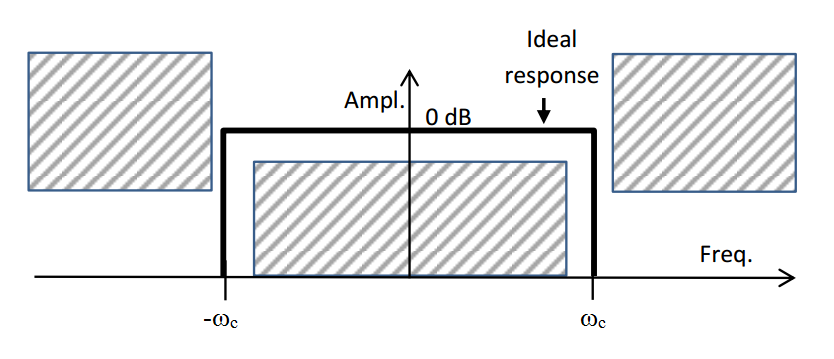
\includegraphics[width=0.6\textwidth]{figures/Ideal_filter.png}
\caption{The ideal frequency response of a lowpass filter.}
\label{fig:IdealFilterApp}
\end{figure}

\section{TLV320AIC3204 setup}


\section{UART setup} \label{UART_setup}

\begin{lstlisting}[language=C, caption = {Initialization of UART},label={listingUartInit}]
// By 16gr640, Spring 2016, AAU
#include "stdio.h"
#include "uart.h"
#include "ezdsp_setup.h"
#define INPUT_FRERQUENCY 100000000

void uartInit(long baudRate)
{
	
	int16 baudRateLSB;
	int16 baudRateMSB;
	
	SYS_EXBUSSEL = 0x1100;
	
	// Setup power management (PWREMU_MGMT). Setting UTRST and URRST to 0
	UART_PWREMU_MGMT = 0x0000;
	
	// Baud rate setup 
	UART_LCR = 0x80; // Setup control line register to change baud rate
	
	// Calculate baud rate
	baudRate = INPUT_FRERQUENCY/(baudRate*16);
	baudRateLSB = (baudRate&0xFF);
	baudRateMSB = ((baudRate>>8)&0xFF);
	
	UART_DLL = baudRateLSB; // Baud rate = 9600
	UART_DLH = baudRateMSB;
	UART_LCR = 0x00; // Disable control line register to not change baud rate
	
	UART_IER = 0x01;
	
	// Setup FIFO control register. (FIFOEN set first) 
	UART_FCR = 0x07; // Clear FIFO's and activate FIFO mode
	
	// Choosing desired protocol setting in LCR
	UART_LCR = 0x03; // No parity bits and 8 bit length word
	
	// (free bit setting in power management and activate UART)
	UART_PWREMU_MGMT = 0x7FFF; // Go go go
	
}

void uartWrite(char *string)
{
	int16 cnt;
	for(cnt=0;string[cnt]!=NULL;cnt++)
	{
		serialWriteByte = (int16)string[cnt];
	}
}
\end{lstlisting}

\begin{lstlisting}[language=C, caption = {Set a flag high if data available in FIFO},label={listingUartFlag}]
    	if(UART_AVAILABLE == 1)
    	{	
			uartFlag = 1;
		}
\end{lstlisting}

\begin{lstlisting}[language=C, caption = {Read the incomming packet from FIFO buffer},label={listingUartRead}]
		/////// UART READ //////
		if (uartFlag == 1){	
			uartReceiveData[0] = UART_RBR;
			uartReceiveData[1] = UART_RBR;
			uartReceiveData[2] = UART_RBR;
			if ((long)uartReceiveData[0] == (long)uartReceiveData[2])
			{
				switch(uartReceiveData[0])
				{
					case 1:
						gainDown128 = uartReceiveData[1];
						break;
					case 2:
						gainBand128 = uartReceiveData[1];
						break;
					case 3:
						gainBand64 = uartReceiveData[1];
						break;
					case 4:
						gainBand32 = uartReceiveData[1];
						break;
					case 5:
						gainBand16 = uartReceiveData[1];
						break;
					case 6:
						gainBand8 = uartReceiveData[1];
						break;
					case 7:
						gainBand4 = uartReceiveData[1];
						break;
					case 8:
						gainBand2 = uartReceiveData[1];
						break;
					case 9:
						gainBand1 = uartReceiveData[1];
						break;
					case 10:
						volume = uartReceiveData[1];
						break;
					case 11:
						byPass = uartReceiveData[1];
						break;
					default: break;
				}	
			} 
			else 
			{
				uartReceiveData[0] = 0;
				uartReceiveData[1] = 0;
				uartReceiveData[2] = 0;
			}
			uartFlag = 0;
		}	
\end{lstlisting}

\begin{lstlisting}[language=C, caption = {Transmit the RMS values of all bands. Only runs every second time},label={listingUartTransmit}]
		///// UART TRANSMIT RMS //////
		if (uartTransmitFlag == 1){
			serialWriteByte = 1;
			serialWriteByte = RMS64bandValue;
			serialWriteByte = RMS32bandValue;
			serialWriteByte = RMS16bandValue;
			serialWriteByte = RMS8bandValue;
			serialWriteByte = RMS4bandValue;
			serialWriteByte = RMS2bandValue;
			serialWriteByte = RMS1bandValue;
			serialWriteByte = 1;
			uartTransmitFlag = 0;
		} else {
			uartTransmitFlag = 1;
		}
\end{lstlisting}
